\subsection{Modelling abstractions}\label{subsec:abstractions}

In molecular networks in the cell, cascades of chemical and physical interactions enable propagation of 
signals through the network. In this process, the activity of upstream molecules induces a change in the 
concentration or activity of downstream molecules. For many reactions, the values of the kinetic parameters 
are unknown or difficult to collect. This lack of knowledge hampers the feasibility 
of computational models that describe molecular networks in fine mechanistic detail, especially for larger networks.
As a solution to this problem, we propose the construction of models at a higher level of abstraction, 
thereby reducing the number of parameters involved. In choosing a suitable abstraction level, it is important to 
retain enough descriptive power to give a meaningful formal description of the topology and the 
associated dynamic behaviour of biological networks.

As a first abstraction in ANIMO models, the active and inactive forms of each network component 
are represented together by a single node in the network.
Each of these nodes is characterized by its \emph{activity level}, which
represents the fraction of active molecules of that molecular species. When a molecule is known to be 
constitutively active, changes in concentrations of that molecule are treated as changes in its activity level.
Activity levels are discretized into integer variables with a user-defined granularity, ranging from 
Boolean (2 levels) to near-continuous (100 levels).

Detailed biochemical reaction mechanisms are abstracted to \emph{interactions}, which can 
represent either activations ($\rightarrow$) or inhibitions ($\dashv$\hspace{0.1em}). 
This aggregation of elementary reactions into single interaction steps reduces the number of kinetic 
parameters involved, while preserving cause-and-effect relationships.
For example, consider a reaction in which enzyme $E$ phosphorylates and activates substrate $S$, 
transferring a phosphate group from a molecule of ATP to a molecule of $S$. Biochemically, this reaction 
can be represented as
$$
\mbox{\it E} + \mbox{\it S} + \mbox{\it ATP} \rightleftarrows \mbox{\it ES} + \mbox{\it ATP} \rightarrow \mbox{\it ES}^{\mbox{\scriptsize \it P}} + \mbox{\it ADP} \rightleftarrows \mbox{\it E} + \mbox{\it S}^{\mbox{\scriptsize\it P}} + \mbox{\it ADP},
$$
with conservation condition $\mbox{\it S} + \mbox{\it S}^{\mbox{\scriptsize\it P}} = \mbox{constant}$ and $\mbox{\it ATP} + \mbox{\it ADP} = \mbox{constant}$.\\
Under the assumption of ATP constantly being replenished by the cell, this reaction is abstracted in ANIMO to the corresponding interaction
$$
\mbox{\it E} \rightarrow \mbox{\it S}.
$$
Each occurrence of the interaction $E \rightarrow S$ will increase the activity level of $S$ by one discrete step. 
Since the activity level is defined as the active fraction of a molecular species, an increase in the active fraction
implies a decrease in the inactive fraction. Hence, the original conservation condition is automatically  
satisfied.
The interaction rate, $R$, depends on the activity levels of the reactants involved and on a single kinetic
parameter $k$ that is set by the user. 
The three available interaction scenarios can be interpreted as abstracted kinetic rate laws:
\begin{enumerate}
  \item $R = k \times [E]$: the interaction rate depends only on the activity level of the upstream node.
  \item $R = k \times [E] \times [1 - S]$ (activations) or $R = k \times [E] \times [S]$ (inhibitions): the rate 
  depends on the activity levels of both the upstream and downstream participants. Activations depend on the 
  presence of inactive substrate, \emph{[1 - S]}, whereas inhibitions depend on the level of active substrate,
  \emph{[S]}.
  \item $R = k \times [E_1] \times [E_2]$: this scenario can be used when the activation or inhibition
  of a downstream node depends on the simultaneous activity of two upstream nodes. This scenario is comparable to an
  \emph{AND-gate} in Boolean logic.
\end{enumerate}
We will show in Section~\ref{sec:results} that the abstraction proposed here preserves ample
expressivity to capture the dynamic behaviour of a biological network. 


\subsection{Modelling interactions with Timed Automata}\label{subsec:timed-automata}
\def\ta{TA}
\def\tas{TA}

Timed Automata have been shown to be a powerful formalism to model biological processes
~\citep{ta-siebert,bartocci-oscillators,oded-ode-ta-discretization}. A timed automaton consists of locations
and transitions between these locations (see Fig.~\ref{fig:abstraction-mek-erk}), and a system of timed automata can be 
used to model a system of interacting molecules. At any time, each automaton is in a specific location, and together 
these locations represent the current state of the biological system. Each timed automaton can have one or more local clocks
associated to it, allowing temporal control of transitions between locations. These transitions are used to 
represent interactions between molecules. Fast interactions take less time than slow interactions 
to perform an activation or inhibition step. We have previously described in detail how the 
scenarios presented in Section~\ref{subsec:abstractions} can be used to calculate the timing of molecular 
interactions to give a description of network dynamics~\citep{animo-bibe}. Figure~\ref{fig:abstraction-mek-erk}
presents a small example that illustrates the basic properties of \tas. 
This model describes the activation of ERK by MEK\footnote{All acronyms used in this paper
and their corresponding UniProt IDs are listed in Suppl. Sect.~\ref{suppl-sec:names}.}.

\def\mekTA{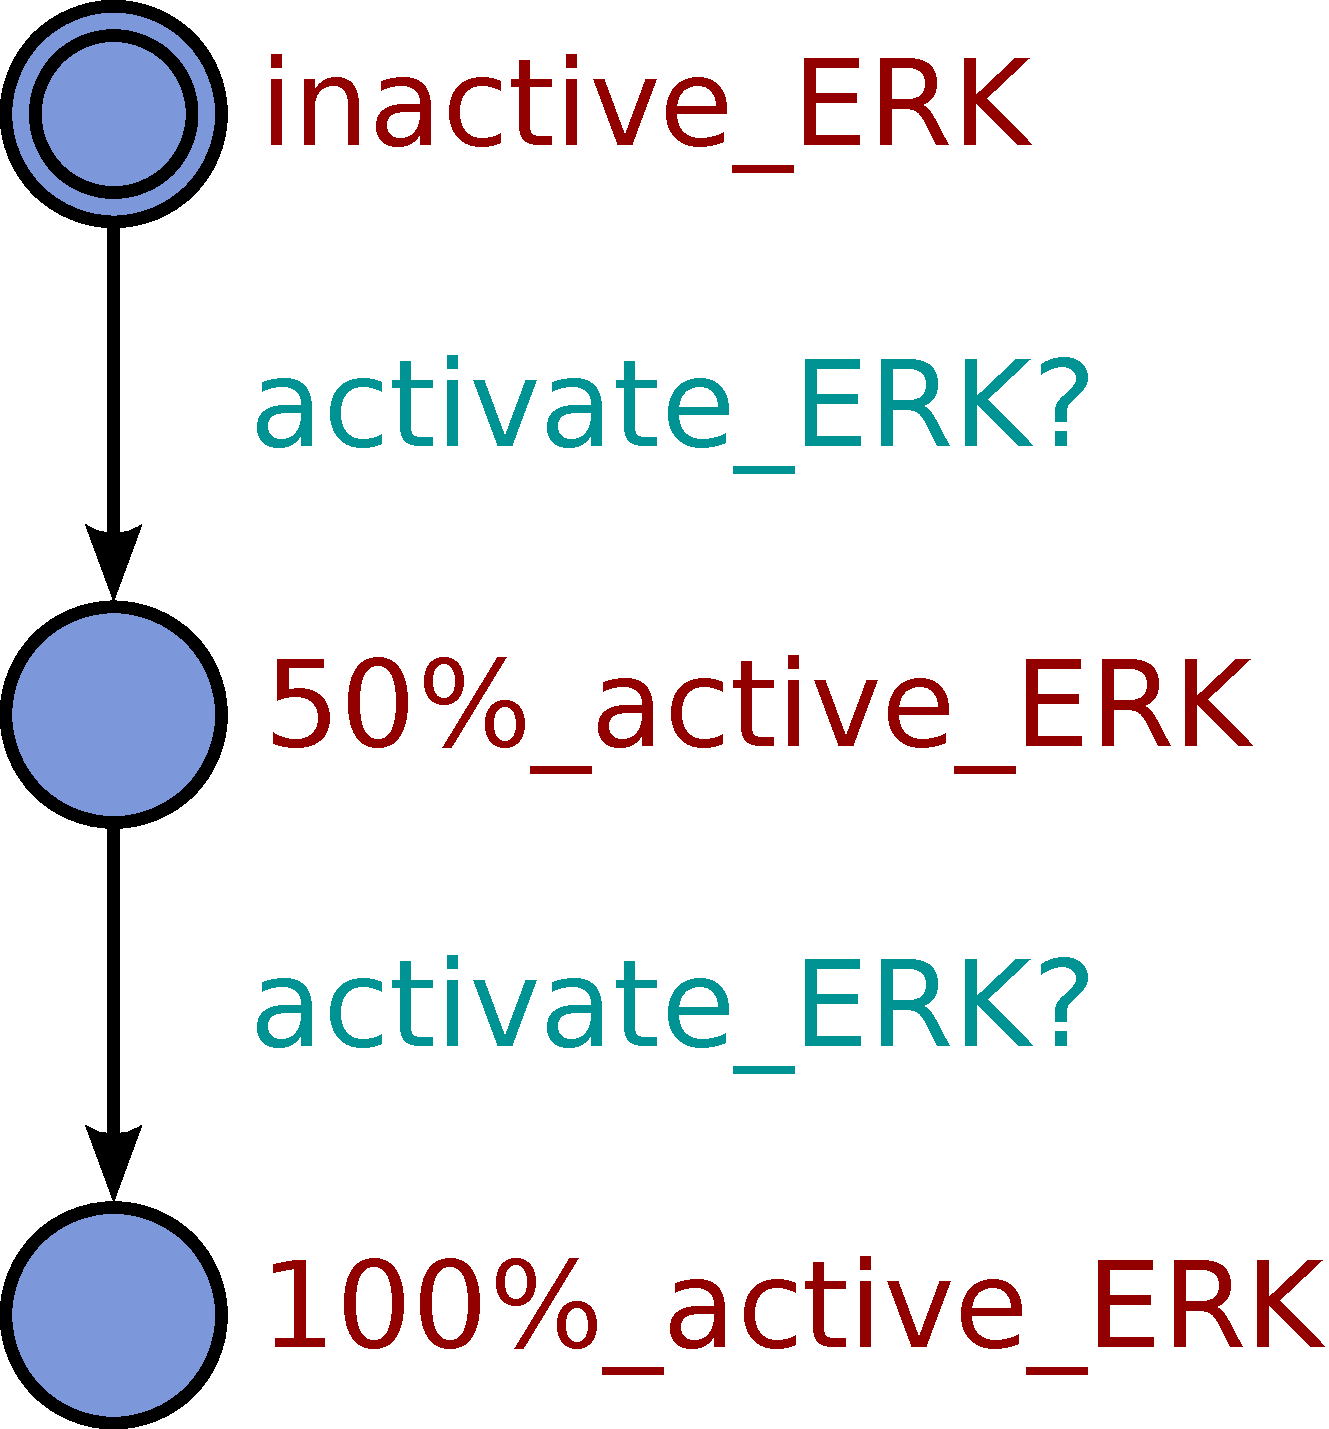
\includegraphics[scale=.098]{images/abstraction_ta_erk3}}
\newlength\mekTAheight
\setlength\mekTAheight{\heightof{\mekTA}}
\begin{figure}[!hb]
%\begin{minipage}{\textwidth}
\begin{center}
\subfloat[\label{subfig:mek-erk}]{\begin{minipage}[c][\mekTAheight]{0.13\textwidth}\begin{center}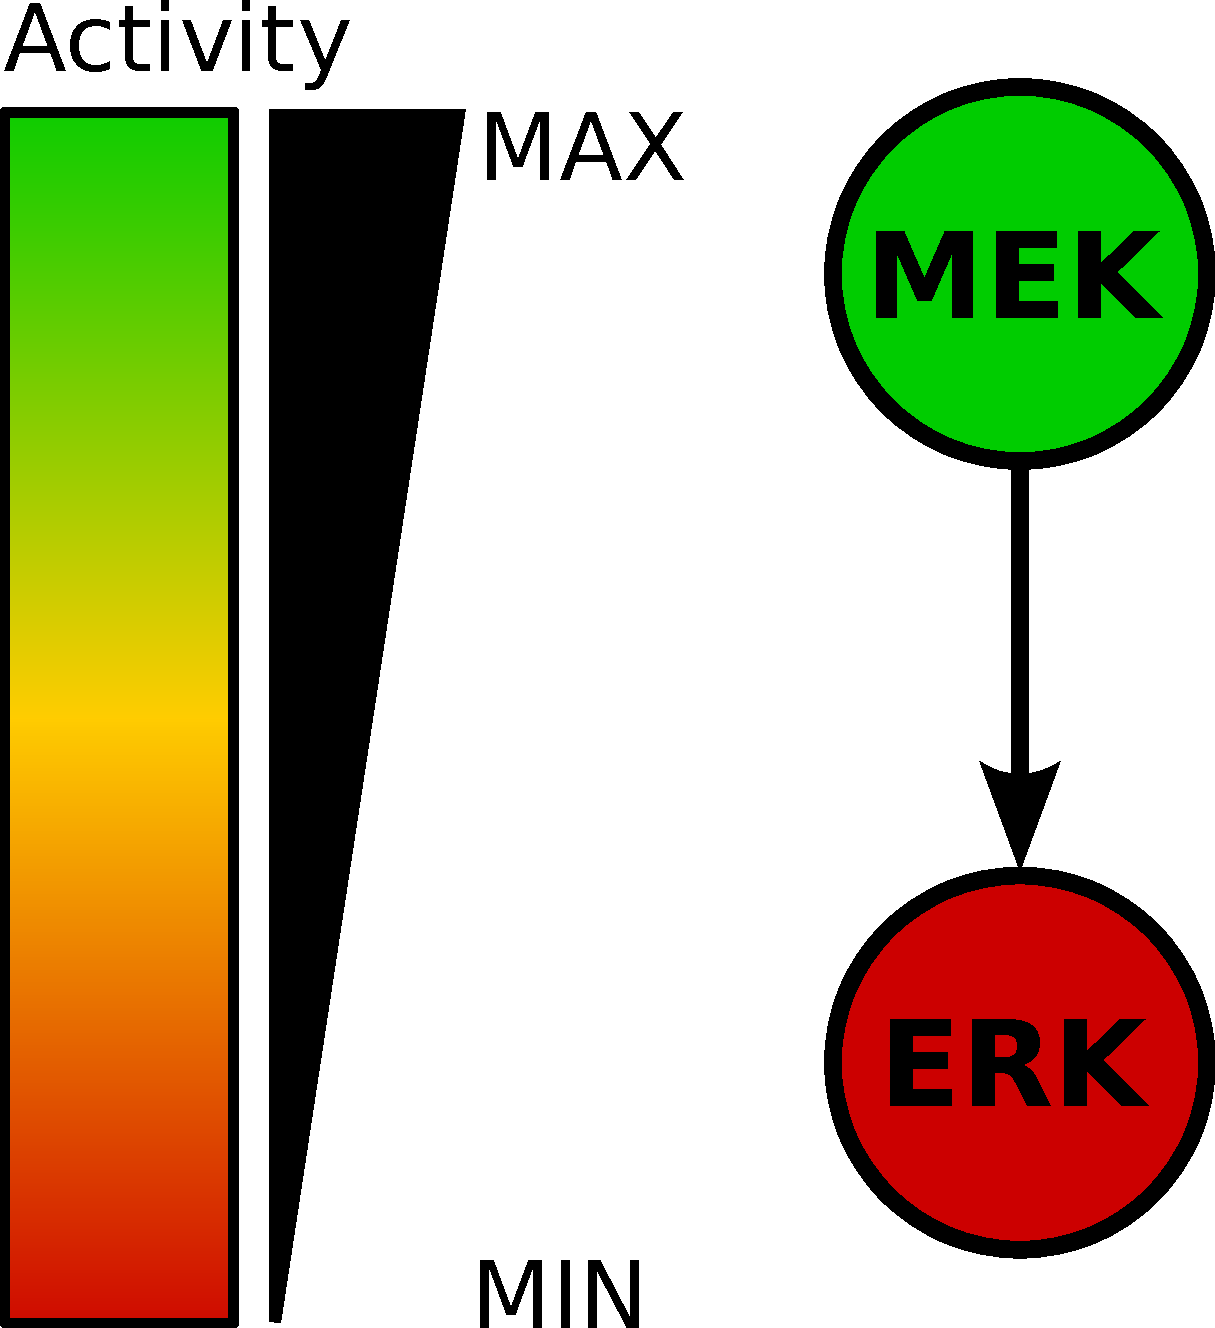
\includegraphics[scale=.098]{images/abstraction_ta_mek-erk3}\end{center}\end{minipage}}
\qquad
\subfloat[\label{subfig:mek}]{\begin{minipage}[c][\mekTAheight]{0.13\textwidth}\begin{center}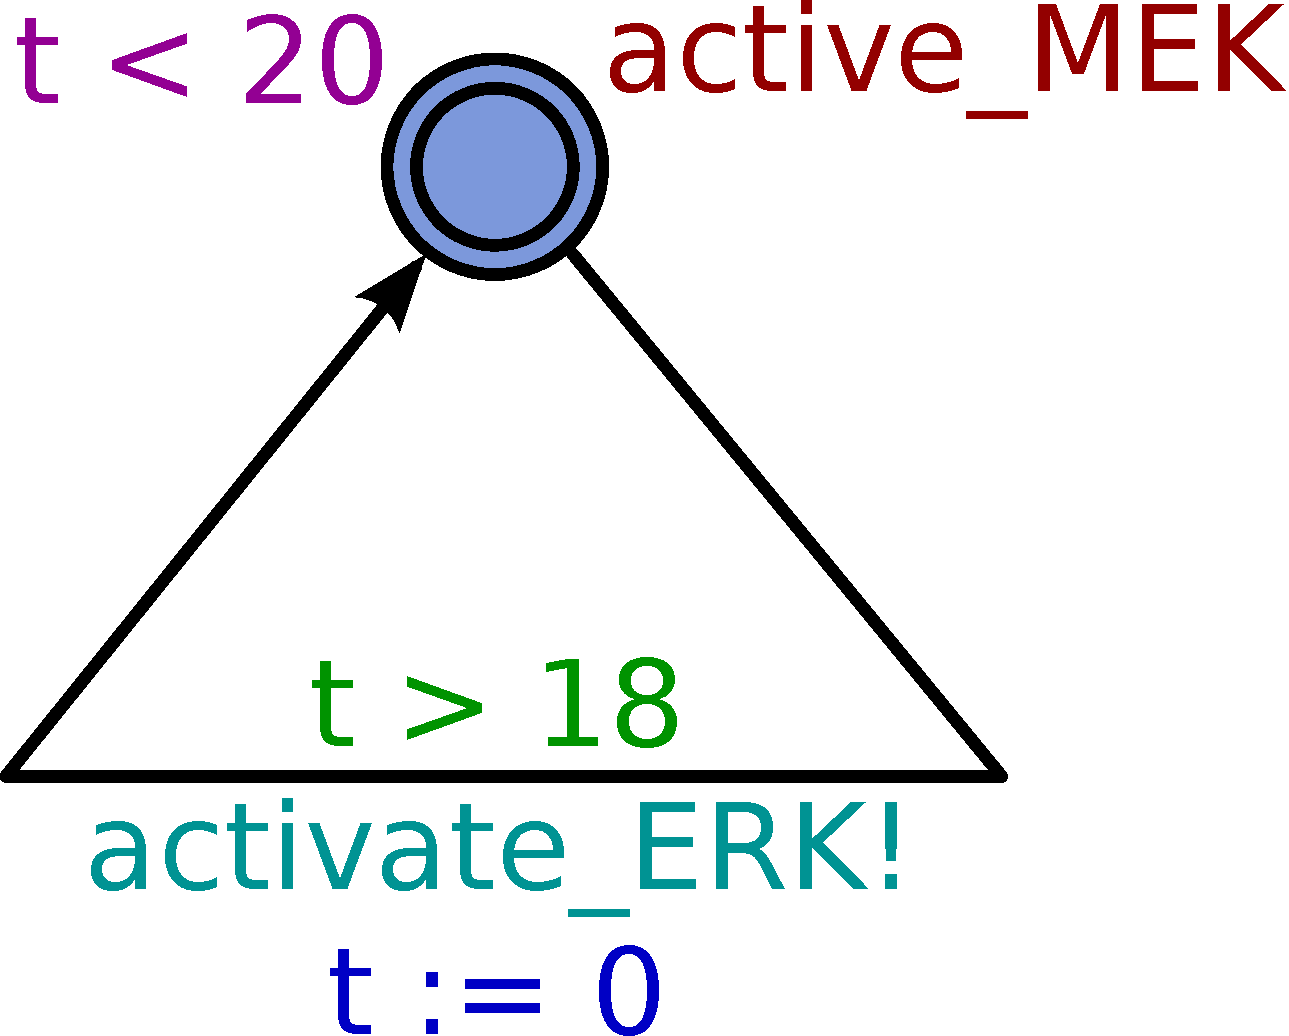
\includegraphics[scale=.098]{images/abstraction_ta_mek}\end{center}\end{minipage}}
\qquad
\subfloat[\label{subfig:erk}]{\begin{minipage}[c][\mekTAheight]{0.14\textwidth}\begin{center}\mekTA\end{center}\end{minipage}}
\end{center}
\caption{Formalization of an activation interaction into a \tas\ model.
{\bf \protect\subref{subfig:mek-erk}}~Classical depiction of a well-studied intracellular signal transduction 
interaction: MEK activates downstream protein ERK.
{\bf \protect\subref{subfig:mek}}~A \ta\ model of MEK, consisting of a single location (circle, active\_MEK) and 
a single transition (arrow). In this example, MEK activity is not regulated and MEK is always active. ${\sf t} < 20$ 
is termed an invariant on the location, allowing residence in this location as long as local
clock time {\sf t} is smaller than $20$ units. ${\sf t} > 18$ is termed a guard on the transition, allowing the
transition to take place when local clock {\sf t} is greater than $18$ units. Together, the invariant and guard
ensure that the transition must take place within the continuous time interval $18 < {\sf t} < 20$. When the
transition takes place, the action {\sf activate\_ERK!} is performed and the local clock is reset, ${\sf t} := 0$.
{\bf \protect\subref{subfig:erk}}~A \ta\ model of ERK, consisting of three locations, {\sf inactive\_ERK}
(the starting location, indicated by a double circle), {\sf 50\%\_active\_ERK} and {\sf 100\%\_active\_ERK},
and two transitions between the locations. Here, ERK has three activity levels: completely inactive, halfway active
and completely active.
A transition will take place when it is possible to synchronize with
the corresponding action {\sf activate\_ERK!} in the MEK automaton.
Each synchronization on channel {\sf activate\_ERK} represents the occurrence of the activating
interaction between MEK and ERK, and allows ERK to eventually become completely active. If we 
replace the time constraints for the occurrence of {\sf activate\_ERK!} with variables depending
on scenario~1 ($R = k \times [MEK]$), the second activation step would have the same time 
constraints as the first activation step, since the interaction rate only depends on MEK. If we use scenario~2
($R = k \times [MEK] \times [1 - ERK]$) instead, the time constraints are doubled after the first activation step, because only
50 \% of inactive ERK is left. The second activation step would then take twice the time of the first step.
}\label{fig:abstraction-mek-erk}
%\end{minipage}
\end{figure}





\subsection{ANIMO}
The modelling approach described in Section~\ref{subsec:abstractions} and Section~\ref{subsec:timed-automata}
is implemented in the
software tool ANIMO (Analysis of Networks with Interactive MOdelling, \citealt{animo-bibe}) as
a plug-in to the network visualization tool Cytoscape~\citep{cytoscape}. The visual interface of Cytoscape
makes the construction, expansion and rewiring of a network topology a fast and user-friendly process. 

When a new node is added to the network, it has to be initialized with the number of activity levels and 
its initial activity. 
For each interaction, a scenario needs to be selected, together with the corresponding kinetic parameter and 
the interaction type: activation or inhibition. All settings can be readily adapted by double clicking, or via a 
table of nodes or interactions. 

ANIMO automatically translates the user input to a \tas\ model, which is then simulated with the model 
checking tool UPPAAL~\citep{uppaal}. The results are subsequently parsed and translated to a graph that shows
the dynamic behaviour of nodes in the network. 
A schematic overview of this process is given in Supplementary Section~\ref{suppl-sec:animo-ta}.
No training or prior knowledge on the use of \tas\ or UPPAAL is needed in order to benefit from ANIMO.
Nevertheless, the \tas\ model and the model checking process in UPPAAL can be accessed when desired by the user.

The dynamic behaviour of a model can be interactively explored by
moving a time slider underneath the graph to highlight time points in a simulation. In the network view,
each node will be coloured according to its activity level at the selected time point. 
Experimental data can be compared to the model by importing and superposing these data 
upon an output graph from the model (Figure~\ref{fig:small-model} B,D,F). The ANIMO user workflow and the 
features described above are illustrated in Suppl. Video 1.






\subsection{Using ANIMO to build a model based on data}\label{subsec:case-study}
To illustrate the process of modelling with ANIMO, we show the construction of a small model based on a 
literature compendium of signal transduction events in HT-29 human colon carcinoma cells~\citep{pathway-compendium}. 
This data set comprises triplicate
measurements of 11 different protein activities or post-translational modification states at 13 time points after
treatment with different combinations of TNF$\alpha$, EGF and insulin.
The data set contains relative protein levels and activities, which is a typical situation in biochemistry.

As a first step, we normalized measurements for each protein to the
maximum value in the complete experiment. This normalization results in a nondimensionalized data set that 
is suitable for use with ANIMO.

In Figure~\ref{fig:small-model}, we show the stepwise construction of a model of a small part of the network that is
able to account for measured variations in activity of IKK, JNK1, MK2, Casp8 and Casp3 upon stimulation with 100~ng/ml TNF$\alpha$.
In this example we aimed for inclusion of a minimum number of nodes in the network, 
while preserving biological relationships.
Multi-step cascades were aggregated into a single step when possible. Parameters for all interactions were 
set manually, and a close match was obtained between the model and the patterns that are present in the dataset.

A more comprehensive model based on the same dataset is presented in Section~\ref{subsec:case-study-larger}.

\def\modelGraphScale{0.2}%0.148}%0.215}
\def\legendGraphScale{0.23}%0.16}
\def\halfGraphScale{0.09}%0.067}%0.1075}
\begin{figure}[!bhtp]
\centering
\begin{tabular}{ll}
\subfloat{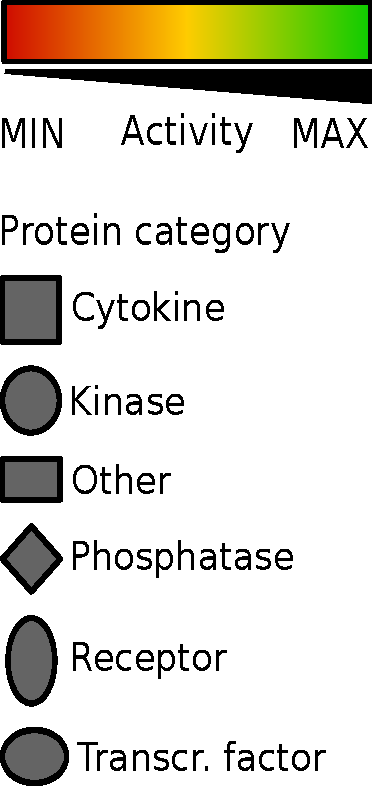
\includegraphics[scale=\legendGraphScale]{images/small-model-1g_legenda}}\addtocounter{subfigure}{-1}\subfloat[\label{fig:small-model-first}]{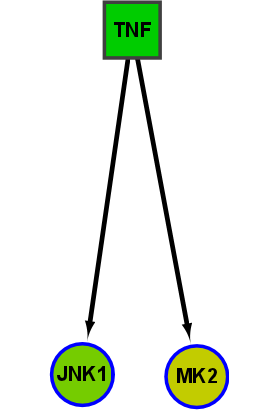
\includegraphics[scale=\modelGraphScale]{images/00-paper-model1f}}
& \subfloat[\label{fig:small-model-first-graph}]{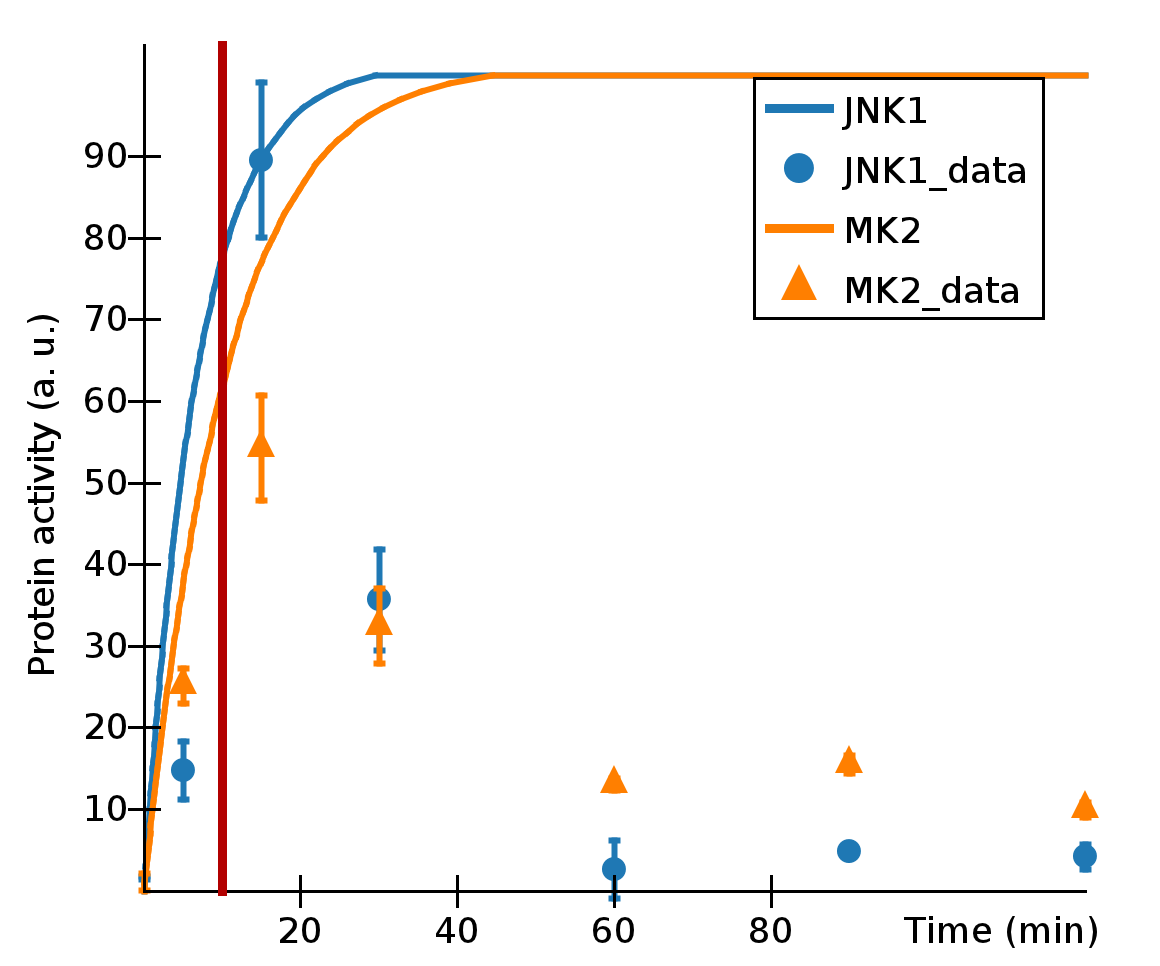
\includegraphics[scale=\halfGraphScale]{images/00-paper-graph1m_riga}} \\[5ex]
\subfloat[\label{fig:small-model-third}]{\qquad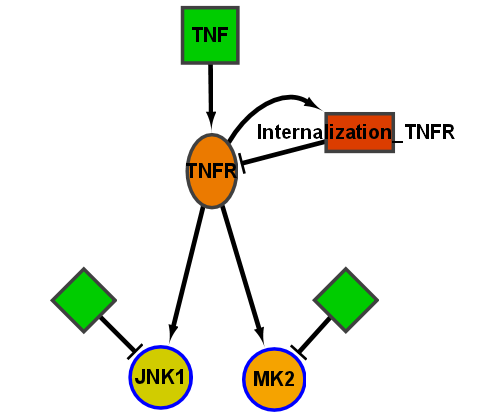
\includegraphics[scale=\modelGraphScale]{images/00-paper-model3f}}
& \subfloat[\label{fig:small-model-third-graph}]{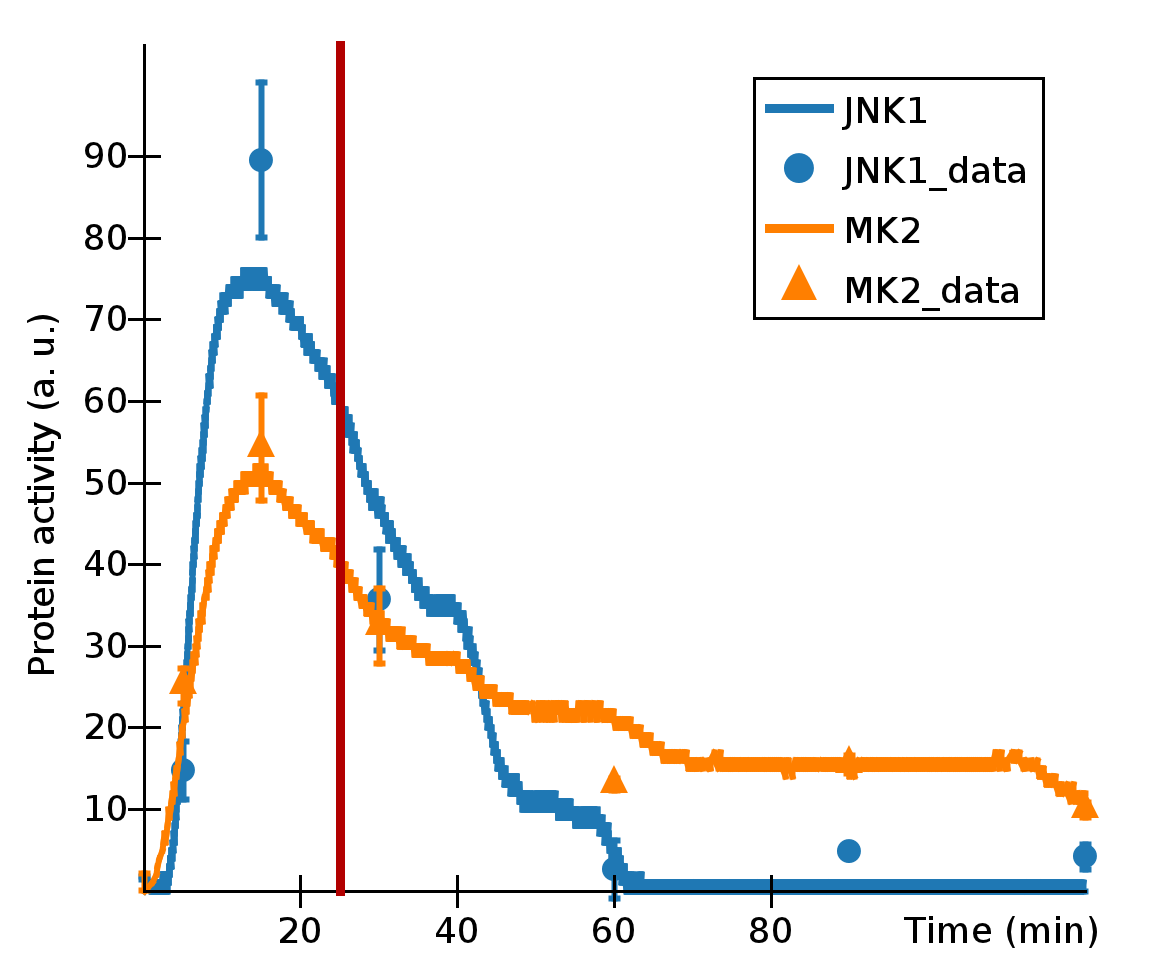
\includegraphics[scale=\halfGraphScale]{images/00-paper-graph3n_riga}} \\[5ex]
\subfloat[\label{fig:small-model-fourth}]{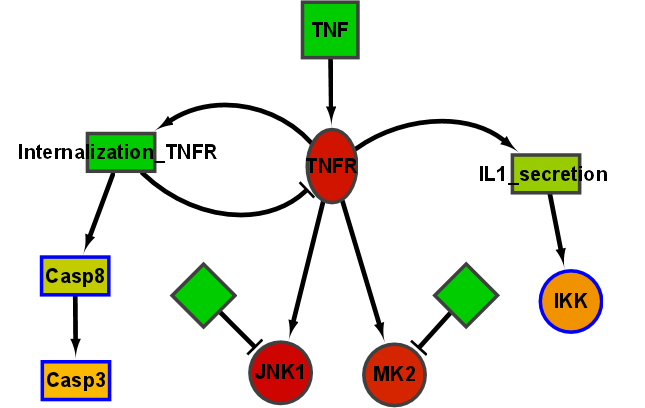
\includegraphics[scale=\modelGraphScale]{images/00-paper-model4g}}
& \subfloat[\label{fig:small-model-fourth-graph}]{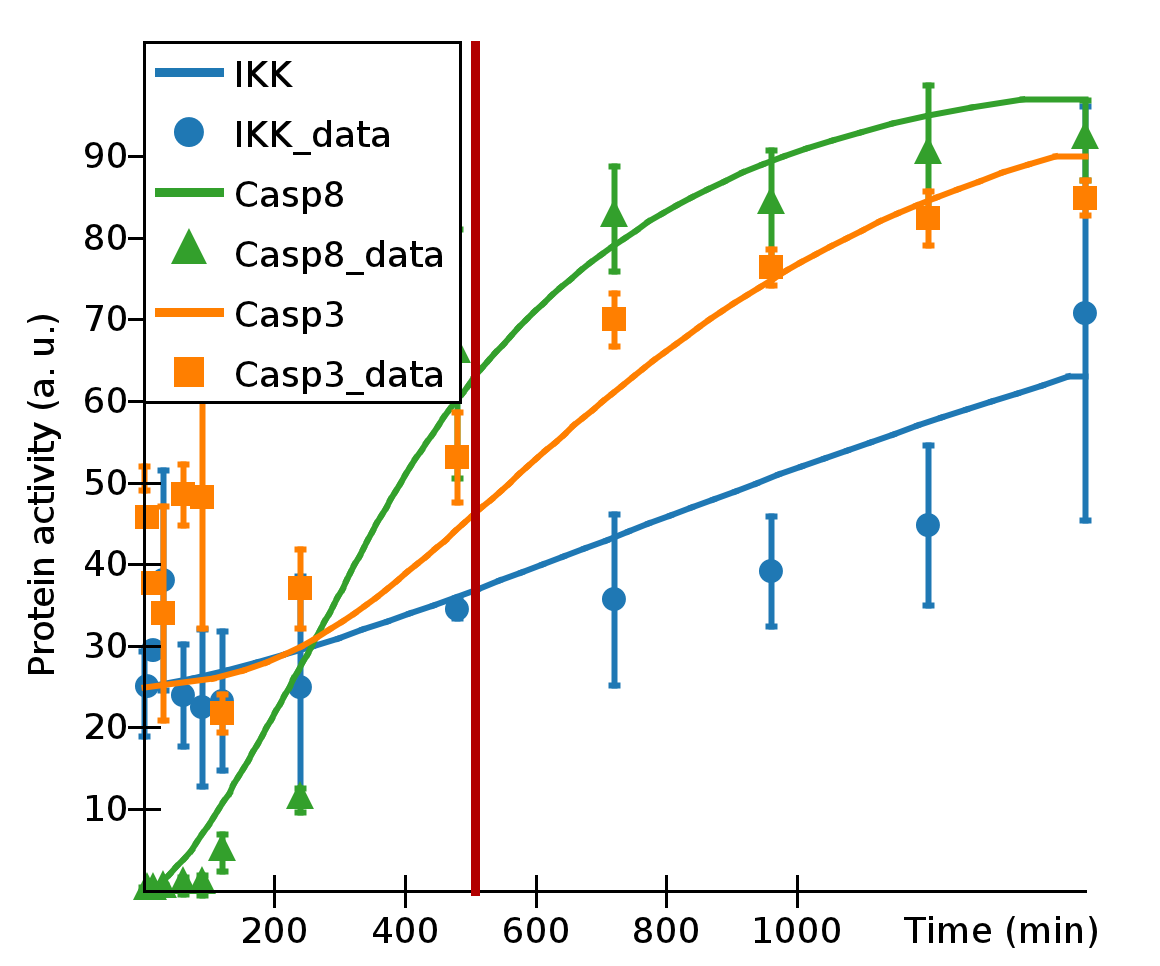
\includegraphics[scale=\halfGraphScale]{images/00-paper-graph4o_riga}}
\end{tabular}
  \caption{
Incremental construction of an ANIMO model of signal transduction
events in human colon carcinoma cells upon stimulation with 100 ng/ml TNF$\alpha$.
Each construction step (top to bottom) is simulated in ANIMO, giving intermediate feedback
useful for the piecewise refinement of the model.
The graphs on the right show the dynamic behaviour of the corresponding models on the left, comparing it to the measured
activity values by~\cite{pathway-compendium} (error bars represent the standard deviation).
On the vertical axis, ``100'' represents the maximum protein activity in the complete experiment.
The red vertical line in each graph indicates a selected time point in the time course. 
Nodes in the corresponding network representation are coloured according to their activity at that time point.
All images in this figure are taken from the ANIMO user interface.
{\bf (\protect\subref*{fig:small-model-first}, \protect\subref*{fig:small-model-first-graph})}~Basic model showing direct activation of JNK1 and MK2 by TNF$\alpha$.
No peak dynamics are observed because no inactivating processes are present.
{\bf (\protect\subref*{fig:small-model-third}, \protect\subref*{fig:small-model-third-graph})}~The model after addition of inactivating phosphatases and a
negative feedback loop that down-regulates TNFR. Note that adding TNFR internalization or phosphatases alone would not be enough to reproduce activity peaks.
{\bf (\protect\subref*{fig:small-model-fourth}, \protect\subref*{fig:small-model-fourth-graph})}~The model after addition of IKK, IL1-secretion (abstracting
the autocrine IL-1 signalling described by~\citealp{pathway-autocrine}), Casp8 and Casp3, showing the late response to TNF$\alpha$ signalling.\\
The {\sf \_{}data} suffix identifies experimental data; all other series are computed by ANIMO.\\
As the data set did not contain values for cleaved caspase-3, but only for its non-cleaved precursor pro-caspase-3,
we computed the {\sf Casp3\_{}data} series as $100\% - [\mbox{\sf pro-Casp3}]$.}\label{fig:small-model}
\end{figure}
